% Capítulo 4 — O sistema (orçamento: ~16 pp)
% O fio condutor: UMA notícia real seguida do princípio ao fim.

\chapter{InvestiGator: o sistema}
\label{cap:sistema}

\section{Vista de conjunto}
\label{sec:sis_vista}

O Capítulo~\ref{cap:metodologia} explicou quatro técnicas isoladas; este mostra-as a trabalhar
juntas, que é onde aparecem os problemas que nenhuma delas tem sozinha.

O sistema chama-se \textbf{InvestiGator} e tem cinco partes, na Figura~\ref{fig:arquitetura}:
\textbf{deteção}, \textbf{recuperação}, \textbf{triagem}, \textbf{explicação} e \textbf{entrega}.
Cada uma tem uma responsabilidade única e passa o resultado à seguinte, o que permite substituir
qualquer delas sem tocar nas outras.

\begin{figure}[ht]
\centering
\begin{tikzpicture}[
  font=\small, >={Stealth[length=2.4mm]},
  cx/.style={draw, rounded corners, align=center, text width=2.6cm, minimum height=1.5cm,
             inner sep=4pt},
  fonte/.style={cx, fill=black!10},
  proc/.style={cx, fill=black!3},
  saida/.style={cx, fill=black!16},
]
  \node[fonte] (p) {\textbf{Preços}\\ \footnotesize fontes gratuitas\\ \footnotesize (com alternativas)};
  \node[fonte, below=6mm of p] (n) {\textbf{Notícias}\\ \footnotesize API gratuita\\ \footnotesize por empresa};
  \node[fonte, below=6mm of n] (h) {\textbf{Histórico}\\ \footnotesize casos antigos\\ \footnotesize com impacto medido};

  \node[proc, right=0.8cm of p] (det) {\textbf{Deteção}\\ \footnotesize é invulgar?};
  \node[proc, right=0.8cm of n] (rec) {\textbf{Recuperação}\\ \footnotesize já aconteceu?};
  \node[proc, right=0.8cm of h] (tri) {\textbf{Triagem}\\ \footnotesize merece avisar?};
  % A decomposicao e a quarta tecnica e faltava aqui. Tracejada porque so entra no
  % alerta de PRECO: sem movimento do dia nao ha nada para repartir.
  \node[proc, dashed, below=6mm of tri] (dec)
    {\textbf{Decomposição}\\ \footnotesize empresa ou mercado?};

  \node[proc, right=0.9cm of rec, text width=2.8cm] (exp)
    {\textbf{Explicação}\\ \footnotesize monta o texto a\\ \footnotesize partir do que foi\\ \footnotesize calculado};

  \node[saida, right=0.8cm of exp, yshift=9mm] (tg) {\textbf{Telegram}\\ \footnotesize alerta no telemóvel};
  \node[saida, right=0.8cm of exp, yshift=-9mm] (web) {\textbf{Página web}\\ \footnotesize consultar quando\\ \footnotesize apetecer};

  \draw[->] (p) -- (det);
  \draw[->] (n) -- (rec);
  \draw[->] (h) -- (tri);
  \draw[->] (h.east) -- ++(0.35,0) |- (rec.west);
  \draw[->] (det.east) -- ++(0.4,0) |- (exp.west);
  \draw[->] (rec) -- (exp);
  \draw[->] (tri.east) -- ++(0.4,0) |- (exp.west);
  \draw[->, dashed] (p.south west) -- ++(-0.35,0) |- (dec.west);
  \draw[->, dashed] (dec.east) -- ++(0.55,0) |- (exp.west);
  \draw[->] (exp.east) -- ++(0.35,0) |- (tg.west);
  \draw[->] (exp.east) -- ++(0.35,0) |- (web.west);
\end{tikzpicture}
\caption[Arquitetura do sistema]{As cinco partes do InvestiGator. À esquerda, de onde vêm os dados;
ao centro, as quatro técnicas do capítulo anterior mais o motor que compõe o texto; à direita, as
duas formas de o utilizador receber o resultado. A \textbf{decomposição} está a tracejado porque é
a única que não corre em todos os alertas: só entra no de preço, já que sem movimento do dia não
há nada para repartir.}
\label{fig:arquitetura}
\end{figure}

Há uma regra de desenho que atravessa tudo isto e que convém enunciar já: \textbf{a explicação é
montada a partir dos objetos que foram calculados}, e nunca escrita à parte. Se o detetor calculou
um $z$ de $+7.61$, é esse número que aparece no texto. Não há um sítio onde alguém escreva a frase e
outro sítio onde alguém calcule o valor, porque, se houvesse, os dois podiam divergir sem
ninguém dar por isso.

\section{De onde vêm os dados}
\label{sec:sis_dados}

Uma restrição fundadora deste trabalho é usar \textbf{apenas fontes gratuitas}. Não foi por
comodidade: é o que torna o sistema utilizável por quem ele serve. Um investidor que já acha caro
pagar comissões não vai subscrever um terminal financeiro.

Isso obriga a três decisões de engenharia.

\paragraph{Preços: uma cadeia, não uma fonte.}
As fontes gratuitas de preços falham com regularidade, seja bloqueando por excesso de pedidos, seja
respondendo com erro, seja simplesmente não tendo ainda o dia de hoje. Em vez de depender de uma, o
sistema tenta várias por ordem e fica pela primeira que responde, registando sempre qual delas
serviu, porque saber de onde veio um número faz parte de o poder explicar.

\paragraph{Notícias: por empresa, e filtradas à entrada.}
As notícias vêm de uma API gratuita, empresa a empresa, e o que chega é muito e é sujo: listas
automáticas de ``os dez maiores movimentos do dia'', textos que mencionam a empresa apenas de
passagem, comunicados de escritórios de advogados. Antes de tudo o resto, portanto, um filtro exige
que a notícia \textbf{nomeie mesmo a empresa} e rejeita os padrões conhecidos de texto automático.

\paragraph{Histórico: um conjunto de dados público, alinhado com preços.}
Para responder à pergunta ``já aconteceu antes?'' é preciso um passado. Usa-se o \gls{FNSPID}
\autocite{dong2024fnspid}, um conjunto público de notícias financeiras, alinhado com os preços
correspondentes. Desse alinhamento nascem cerca de 80 mil casos entre 2018 e 2023, cada um com o
que o preço fez a seguir, e é sobre eles que a recuperação é \emph{avaliada} no
Capítulo~\ref{cap:avaliacao}.

Convém separar isso do que o sistema \emph{implantado} consulta, porque não é o mesmo ficheiro. Em
produção a base de casos é um ano de notícias reais recolhidas pelo próprio sistema, com o impacto
medido da mesma maneira: são $38\,214$ casos. Um serve para medir se o método funciona, o outro é o que
está a correr.

\section{As peças que não são minhas}
\label{sec:sis_pecas}

O sistema assenta em serviços de terceiros, todos gratuitos, e cada um é uma dependência e um
limite. As notícias vêm de três fontes complementares, comparadas na Secção~\ref{sec:sis_fontes};
os preços vêm de uma cadeia de quatro alternativas tentadas por ordem fixa, porque nenhuma fonte
gratuita de preços é fiável sozinha e sem a cadeia um dia de bloqueio seria indistinguível de um
dia em que o mercado não abriu; o registo guarda sempre qual delas serviu, porque a origem de um
número faz parte de o poder explicar. A representação de frases usa um codificador pré-treinado,
escolhido por medição contra quatro alternativas (Secção~\ref{sec:av_alternativas}), e a entrega
usa a interface de robô do Telegram. Duas candidaturas foram rejeitadas por medição e não por
argumento: uma fonte de preços que responde com verificação anti-robô, e uma de notícias que não
permite consulta por empresa.

\subsection{Porquê três fontes de notícias, e não a melhor}
\label{sec:sis_fontes}

O sistema começou com uma fonte só, e a pergunta natural é se acrescentar mais compensa. A resposta
não é ``mais é melhor'': é preciso medir, porque cada fonte custa pedidos e uma fonte generosa mas
mal etiquetada não acrescenta nada de aproveitável.

O critério também não pode ser quantas notícias cada uma devolve, mas quantas \textbf{sobrevivem ao
filtro de relevância} que já está em produção, porque tudo o que é rejeitado à entrada não chega a
existir para o sistema. A Tabela~\ref{tab:sis_fontes} mede exatamente isso, sobre as doze empresas
e três dias.

\begin{table}[!htbp]
\caption[As três fontes, medidas]{O que cada fonte gratuita entrega depois do filtro de
relevância. A última coluna é a que decide se compensa somar: quantos títulos cada uma traz
que \emph{nenhuma} das outras traz. \textbf{Essa coluna é um limite superior}, e a razão é a
regra de comparação: dois títulos só contam como o mesmo se coincidirem depois de passarem a
minúsculas e de se lhes tirar a pontuação. Duas fontes que reescrevam o mesmo acontecimento por
outras palavras contam como dois títulos exclusivos, e é isso que explica a sobreposição
observada ser tão pequena. Fazer a comparação por \emph{significado} usaria a técnica que o
sistema já tem, e é o item~5 da Secção~\ref{sec:con_futuro}.}
\label{tab:sis_fontes}
\centering
\small
\begin{tabular}{L{0.20\textwidth} C{0.12\textwidth} C{0.11\textwidth} C{0.13\textwidth}
                C{0.12\textwidth} C{0.13\textwidth}}
\toprule
\tabhead{Fonte} & \tabhead{Relevantes} & \tabhead{Precisão} & \tabhead{Frescura} &
\tabhead{Cobertura} & \tabhead{Exclusivas} \\
\midrule
Finnhub & $432$ & $\mathbf{35\%}$ & $15.8$ h & $\mathbf{12/12}$ & $401$ \\
Alpha Vantage & $141$ & $24\%$ & $\mathbf{9.3}$ \textbf{h} & $\mathbf{12/12}$ & $119$ \\
Polygon & $429$ & $27\%$ & $52.6$ h & $8/12$ & $\mathbf{418}$ \\
\bottomrule
\end{tabular}
\end{table}

Três fontes gratuitas com \textbf{três forças diferentes}, e é isso, e não o volume, que justifica
somá-las:

\begin{itemize}
  \item o \textbf{Finnhub} etiqueta melhor e cobre todas as empresas;
  \item a \textbf{Alpha Vantage} é a mais fresca, com $9.3$ horas de mediana contra $15.8$, e a
        frescura é exatamente o que ataca a queixa de os alertas chegarem tarde;
  \item o \textbf{Polygon} traz mais títulos exclusivos do que qualquer outra fonte, incluindo o
        Finnhub, mas com $52.6$ horas de mediana. Serve para \emph{encher a base de casos}, não
        para alertar, e é assim que está a ser usado.
\end{itemize}

Juntas dão \textbf{$970$} títulos relevantes distintos, contra os $432$ do Finnhub sozinho: mais
$125\%$. Para as empresas menos cobertas a diferença é maior ainda, e são precisamente essas as que
o sistema quase nunca conseguia comentar.

Há ainda um segundo motivo, que não é de volume: quando uma fonte falha ou bloqueia, as outras
respondem. É a mesma razão pela qual os preços já vinham de uma cadeia e não de uma fonte só.

\paragraph{O que isto não compra.}
Latência garantida. As três publicam com atrasos próprios, e o ganho num caso concreto depende de
qual delas viu a história primeiro. A frescura mediana melhora, e isso está medido; afirmar que os
alertas passam a chegar mais cedo em geral exigiria voltar a medir a latência ponta a ponta ao fim
de algumas semanas, e isso ainda não foi feito.

\paragraph{Nada disto é escolhido por gosto sem prova.}
Duas destas linhas mudaram por \emph{medição} e não por opinião: o Stooq foi despromovido depois de
se ver o que devolve, e o modelo de vetores foi comparado com três alternativas antes de ficar. As
restantes são escolhas de restrição: são as que cabem em ``apenas fontes gratuitas''.

\section{O caminho de uma notícia, do princípio ao fim}
\label{sec:sis_caminho}

Esta é a secção central do capítulo, e segue \textbf{uma notícia real}: um alerta que o canal
enviou a 12 de julho de 2026 sobre a Meta.

\begin{quote}
\emph{``Mark Zuckerberg Said Meta's AI Bets `Haven't Come to Fruition Yet' as Shares Fell 5\%''}
\end{quote}

A Figura~\ref{fig:caminho} mostra as nove etapas.

\begin{figure}[ht]
\centering
\begin{tikzpicture}[
  font=\footnotesize, >={Stealth[length=2mm]},
  et/.style={draw, rounded corners, align=center, text width=2.15cm, minimum height=1.15cm,
             fill=black!3},
  porta/.style={et, dashed, fill=orange!10},
  n/.style={font=\bfseries\footnotesize, text=black!45},
]
  \node[et] (a) {recolher\\ notícias};
  \node[porta, right=4mm of a] (b) {nomeia a\\ empresa?};
  \node[porta, right=4mm of b] (c) {é recente?};
  \node[et, right=4mm of c] (d) {procurar\\ casos\\ parecidos};
  \node[porta, below=7mm of d] (e) {evidência\\ forte?};
  \node[porta, left=4mm of e] (f) {merece\\ avisar?};
  \node[porta, left=4mm of f] (g) {já avisei\\ hoje?};
  \node[et, left=4mm of g] (h) {montar a\\ explicação};
  \node[et, below=7mm of h, fill=black!16] (i) {enviar e\\ registar};

  \foreach \x/\i in {a/1, b/2, c/3, d/4} { \node[n, above=0.5mm of \x] {\i}; }
  \foreach \x/\i in {e/5, f/6, g/7, h/8} { \node[n, above=0.5mm of \x] {\i}; }
  \node[n, above=0.5mm of i] {9};

  \draw[->] (a) -- (b); \draw[->] (b) -- (c); \draw[->] (c) -- (d);
  \draw[->] (d) -- (e); \draw[->] (e) -- (f); \draw[->] (f) -- (g); \draw[->] (g) -- (h);
  \draw[->] (h) -- (i);
\end{tikzpicture}
\caption[As nove etapas de um alerta]{As nove etapas. As caixas a tracejado são \textbf{portas}: em
qualquer uma delas a notícia pode ser descartada e o sistema fica calado. Nove em cada dez
varreduras acabam assim.}
\label{fig:caminho}
\end{figure}


Os valores desse alerta, etapa a etapa: o título nomeia a empresa e não corresponde a nenhum padrão
de texto automático; tem menos de dois dias; os três precedentes mais próximos são Microsoft
2023-11-07 ($0.46$), Nvidia 2023-08-02 ($0.51$) e Nvidia 2023-09-21 ($0.46$), e a melhor semelhança
fica acima do chão de $0.45$; o modelo de triagem atribui $54\%$; é o primeiro alerta da empresa
nesse dia. A mensagem é composta a partir dos objetos calculados e registada.

A etapa 4 merece atenção, e a razão está no que ela devolve. Os três
casos recuperados são de \textbf{outras empresas} (duas da Nvidia e uma da Microsoft), e o
sistema mostra-os na mesma. É deliberado: se a pergunta é ``já houve notícias como esta?'', a
resposta não tem de vir da mesma empresa. Notícias sobre investimento em inteligência artificial numa
tecnológica grande são comparáveis entre si.

E os desfechos foram \textbf{em sentidos opostos}: $+2.70\%$, $-3.87\%$ e $+5.05\%$. O sistema
mostra os três, um a um, exatamente por isso. Se mostrasse só a média, esconderia o que mais
importante que há para saber: que casos parecidos deram resultados diferentes.

\section{O caminho de um movimento de preço}
\label{sec:sis_mercado}

O segundo gatilho é bastante mais curto: todos os dias, depois do fecho, o sistema calcula o
\emph{z}-score de cada empresa da lista, como na Secção~\ref{sec:met_zscore}, e basta que um deles
ultrapasse o limiar para haver alerta.

É também aqui, e só aqui, que entra a segunda técnica do Capítulo~\ref{cap:metodologia}. Ao alerta
de preço é acrescentada uma linha com a \textbf{repartição do movimento}, calculada como a
Secção~\ref{sec:met_decomposicao} descreve, do género
\emph{``NFLX $-2.11\%$ hoje $=$ $-0.08\%$ mercado $\cdot$ $-0.32\%$ setor $\cdot$ $-1.71\%$ da
própria empresa''}, seguida de uma frase em palavras que nomeia a maior parcela. É a resposta à
segunda das três perguntas fundadoras, entregue em números dentro da mensagem.

Não aparece no alerta de notícia, e a razão é que a repartição é do \emph{movimento do dia}: sem
movimento não há o que repartir. Quando a estimação da sensibilidade ao mercado falha, a linha sai
na mesma mas diz que assumiu sensibilidade $1.0$ e que a repartição é indicativa, em vez de calar
a incerteza.

Duas capacidades foram acrescentadas depois de o sistema estar a funcionar, e ambas por observação:

\begin{description}
  \item[Níveis de severidade.] Um $z$ de $1.6$ e um $z$ de $3.2$ não são a mesma coisa, e o texto do
        alerta passou a distingui-los em palavras (``assinalável'', ``forte'', ``extremo'') em
        vez de dar o mesmo aviso aos dois.
  \item[Comparação com os pares.] Um alerta que diz ``a empresa caiu 8\%'' sem dizer que o setor
        inteiro caiu é enganador. O sistema passou a olhar para as outras empresas do mesmo setor no
        mesmo dia, e a dizê-lo.
\end{description}

Esta segunda correção veio de ler os primeiros trinta alertas enviados. Em nove deles o texto
\textbf{contradizia-se}: uma linha dizia que o movimento parecia ser do setor inteiro, e duas linhas
abaixo a repartição dizia que a maior parte pertencia à empresa. As duas linhas estavam certas
isoladamente: a comparação com os pares olhava apenas para a \emph{direção} do movimento dos
vizinhos, nunca para a sua \emph{dimensão}. Passou a olhar para as duas.

\section{As portas: quando o sistema decide calar-se}
\label{sec:sis_portas}

Porque avisar de tudo é o mesmo que não avisar de nada. Se o canal enviar quinze mensagens por dia,
a pessoa deixa de as ler, e o sistema perde o único valor que tinha para dar.

As cinco portas da Figura~\ref{fig:caminho} existem precisamente para isso, e o efeito conjunto
delas é grande: numa janela medida em produção, das \textbf{944} notícias relevantes que entraram
saíram \textbf{42} alertas, ou seja cerca de uma em cada vinte e duas.

Vale a pena ver isto num dia concreto, com os números lidos do registo do próprio sistema. A
Tabela~\ref{tab:sis_funil} mostra as avaliações registadas a 15 de agosto de 2026.

\begin{table}[!htbp]
\caption[O funil de um dia real]{Onde morreram as avaliações registadas a 15 de agosto de 2026.
São as $5\,060$ que o registo continha no momento em que foi lido, o que é \emph{parte} de um dia e
não o dia inteiro. O que se lê aqui são proporções, não totais. A coluna da direita é a parte que
interessa.}
\label{tab:sis_funil}
\centering
\small
\begin{tabular}{L{0.30\textwidth} r L{0.42\textwidth}}
\toprule
\tabhead{Onde morreu} & \tabhead{Avaliações} & \tabhead{O que é} \\
\midrule
Sem precedente forte & $2\,994$ & nenhum caso passado acima do chão de semelhança \\
Abaixo do piso da triagem & $1\,194$ & o modelo pontuou abaixo do mínimo \\
Piso escalonado & $269$ & o segundo alerta do dia exigia pontuação mais alta \\
A mesma história & $249$ & já contada por outras palavras \\
Orçamento esgotado & $21$ & o dia já tinha gasto os cinco alertas \\
Sobreviveu às portas & $333$ & \textbf{ver a ressalva} \\
\midrule
\textbf{Mensagens entregues} & \textbf{5} & o orçamento do dia, gasto por inteiro \\
\bottomrule
\end{tabular}
\end{table}

\paragraph{Uma etapa que não estava instrumentada.}
Cinco mil avaliações e cinco mensagens: a proporção está certa e é o comportamento pretendido. Mas
a linha dos $333$ não queria dizer o que parecia. O sistema reavalia os mesmos títulos de $60$ em
$60$ segundos, e um título que já tinha sido entregue nesse dia voltava a passar todas as portas
a cada minuto. Era travado no fim, por uma verificação de ``isto já foi enviado'' que
\textbf{não estava registada como uma etapa}, ao contrário de todas as outras.

Resultado: a vista que existe para tornar as decisões do sistema inspecionáveis dizia
``alerta enviado'' $333$ vezes num dia em que enviou $5$ mensagens. Não é um erro de contagem
inofensivo: é a mesma classe de defeito que a tabela abaixo documenta para as outras portas,
sobrevivendo na única que ficou por instrumentar.

Está corrigido: a supressão passou a ser uma etapa com nome próprio, como as outras, e existe um
teste que falha se voltar a desaparecer. Os números da tabela são os de \emph{antes} da correção,
e sabe-se que são: o registo não contém uma única linha da etapa nova, quando $333$ sobreviveram às
portas e apenas $5$ foram enviadas.

Cada porta tem uma constante associada, e é justo perguntar de onde vêm esses números. A
Tabela~\ref{tab:sis_portas} responde, incluindo quando a resposta é ``foi escolhido''.

\begin{table}[!htbp]
\caption[As portas e as suas constantes]{Cada porta, e de onde vem o valor que usa. A primeira
não tem valor nenhum, porque é uma regra de texto e não um limiar. A porta ``já avisei hoje'' não aparece porque não tem constante nenhuma, e o
orçamento diário aparece porque, apesar de atuar depois das portas da figura, é hoje quem
verdadeiramente corta. Distinguir ``derivado'' de ``escolhido'' é uma
questão de honestidade: os dois casos defendem-se de maneiras diferentes.}
\label{tab:sis_portas}
\centering
\small
\begin{tabular}{L{0.22\textwidth} L{0.16\textwidth} p{0.50\textwidth}}
\toprule
\tabhead{Porta} & \tabhead{Valor} & \tabhead{De onde vem} \\
\midrule
Nomeia a empresa & --- & Regra escrita depois de ler os primeiros alertas e ver o que passava. \\
É recente & 2 dias & Escolhido: cobre um fim de semana. \\
Evidência forte & $0.45$ & \textbf{Escolhido}, e é a porta mais agressiva de todas (ver abaixo). \\
Merece avisar & $50\%$ & \textbf{Derivado} de uma análise de custos, que dá $0.49$ quando falhar um
movimento e dar um falso alarme custam o mesmo; o valor implantado foi arredondado à mão para
$0.50$. \textbf{Hoje já não veta}: serve para \emph{ordenar} as candidatas, e quem corta é o
orçamento diário. \\
Orçamento diário & 5/dia & Escolhido, e é hoje o verdadeiro controlo de volume. \textbf{Mas} os cinco
lugares são gastos \textbf{por ordem de chegada}, e não pelas cinco melhores do dia: a decisão é
tomada de ciclo em ciclo, sem saber o que a tarde ainda traz. A pontuação ordena as candidatas
\emph{do mesmo ciclo}, e é o piso escalonado que encarece cada lugar seguinte. Veio corrigir um
teto de duas por empresa, que limitava cada nome e não o total. \\
\addlinespace
Piso escalonado & primeiro livre; segundo $0.64$ & A configuração conserva os valores derivados
$0.49$ e $0.64$, mas, com o orçamento global ligado, o código ignora explicitamente o primeiro: o
primeiro alerta do dia de cada empresa não tem piso de triagem. O segundo exige $0.64$. Assim a
escada atua apenas como anti-fadiga dentro da mesma empresa e não volta a excluir à partida nomes
cuja pontuação-base é baixa. \\
\bottomrule
\end{tabular}
\end{table}

O chão de semelhança merece um parágrafo próprio, porque é a porta que trava mais casos e a que
tem a justificação mais fraca. Numa varredura medida, quando a lista vigiada ainda tinha dez nomes,
sete deles foram travados exatamente ali, e quatro por $0.04$ ou menos de diferença. Testei depois se um valor mais alto de
semelhança correspondia a precedentes mais informativos, e \textbf{não corresponde}: a concordância
de direção entre o caso passado e o caso atual fica ao nível do acaso dos dois lados do limiar. A
conclusão honesta é que este número serve para \emph{controlar o volume} de alertas e para garantir
coerência de tema, e não para escolher casos que preveem melhor. Fica dito assim.

\section{Como o alerta é explicado}
\label{sec:sis_explicacao}

O alerta não é uma frase. É uma pequena estrutura, sempre com as mesmas partes e sempre pela mesma
ordem:

\begin{enumerate}
  \item \textbf{o facto}: o que aconteceu, em números, e a fonte;
  \item \textbf{os casos passados}: um a um, com data, semelhança e o que se seguiu a cada um;
  \item \textbf{a ressalva}: que isto é história observada e não uma previsão;
  \item \textbf{a estimativa}: a probabilidade de o mercado reagir, e nunca em que direção.
\end{enumerate}

A ordem importa, e cada extremo foi escolhido. A pessoa lê primeiro o que aconteceu e só depois a
estatística, porque é assim que uma pessoa pensa; um alerta que abre com ``$z = 2.65$'' perde o
leitor na primeira linha. E a estimativa fica em \textbf{último}, porque é o único número da
mensagem que olha para a frente: quem parar de ler antes dela fica com factos e com histórico, que
é exatamente o que este trabalho quer entregar.

No alerta de movimento de preço a primeira parte traz também a razão estatística, em linguagem
simples, porque aí o que aconteceu \emph{é} o movimento; no alerta de notícia esse lugar é
ocupado pelo título e pela ligação para o artigo.

Importa também a \emph{quantidade}. O sistema mostra três precedentes e não os trinta que encontrou,
e essa não é uma decisão de espaço no ecrã: a investigação sobre explicação estabelece que as pessoas
procuram razões seletivas e contrastivas, e não uma enumeração exaustiva de tudo o que contribuiu
\autocite{miller2019explanation}. Uma lista com trinta casos seria mais completa e menos útil, porque
a pessoa não a leria. Pela mesma razão o alerta exibe as quantidades exatas por detrás da decisão e
não o cálculo inteiro que as produziu.

A Figura~\ref{fig:sis_alerta} mostra um alerta \textbf{tal como foi entregue}, copiado do registo
do canal. A mesma informação fica disponível numa página web, que serve para consultar o que foi
enviado e, sobretudo, o que \emph{não} foi: é aí que vive o registo das decisões descrito na
Secção~\ref{sec:sis_portas}. A Figura~\ref{fig:sis_pagina} mostra as duas metades, capturadas
da aplicação em funcionamento. A interface em si não é uma contribuição deste trabalho, e por
isso não se descreve aqui o seu desenho; mostra-se porque é o único sítio onde o \emph{silêncio}
do sistema é visível.

A empresa da figura é um caso instrutivo, e o que o torna instrutivo é a discordância entre a
percentagem e a repartição. A ação estava a descer $0.41\%$; o mercado e a própria empresa
estavam ligeiramente em alta, $+0.08\%$ e $+0.07\%$; e o que a puxava para baixo era o
\textbf{setor}, com $-0.56\%$. A percentagem sozinha diz \emph{a Johnson \& Johnson desceu} e
convida a procurar uma razão na empresa, onde não há nenhuma. É esta a diferença que a segunda
pergunta do trabalho existe para tornar visível.

Repare-se ainda que o veredicto termina em \emph{``so far today''}: a captura é de meio da
sessão americana, não de um fecho, e o sistema di-lo em vez de apresentar um número em curso
como se fosse definitivo.


\begin{figure}[ht]
\centering
\begin{tcolorbox}[colback=black!3, colframe=black!35, boxrule=0.4pt, arc=2pt,
                  width=0.97\textwidth, fontupper=\ttfamily\scriptsize]
\textcolor{black!55}{[1]} News alert for AMZN (Amazon) (2026-08-13)\\
\hspace*{1em}"Prediction: Amazon Will Join Apple in the \$4 Trillion Club Before 2030"\\[4pt]
\textcolor{black!55}{[2]} 3 similar past headlines. Their 5-day move ranged -2.73\% to -2.73\%\\
\hspace*{1em}(average -2.73\%):\\
\hspace*{1em}-2.73\% in 5d · AAPL 2026-08-05 (8d ago) · "If You Invested \$100 In Apple\\
\hspace*{2em}Stock 10 Years Ago, You Would Have This Much Today" (sim 0.56)\\
\hspace*{1em}-2.73\% in 5d · AAPL 2026-08-05 (8d ago) · "Apple's Selloff Is Overdone"\\
\hspace*{2em}(sim 0.51)\\
\hspace*{1em}-2.73\% in 5d · AAPL 2026-08-05 (8d ago) · "Apple's Buyback Is Retiring\\
\hspace*{2em}Less Stock Just As The Memory Bill Grows" (sim 0.47)\\[4pt]
\textcolor{black!55}{[3]} 3 of 3 shown cases moved down — topic-similar past cases, not a\\
\hspace*{1em}prediction for this news (an observed pattern, not a forecast).\\
\hspace*{1em}Observed past outcomes after similar news, not a price prediction and\\
\hspace*{1em}not advice.\\[4pt]
\textcolor{black!55}{[4]} Materiality estimate (learned triage): 57\% chance of an unusually\\
\hspace*{1em}large move over the next few days, in EITHER direction — raised by\\
\hspace*{1em}recent volatility (20d) and sector; lowered by today's own move and\\
\hspace*{1em}recent momentum (5d). This estimates whether the market reacts, never\\
\hspace*{1em}which way: it is not a price forecast and not advice.
\end{tcolorbox}
\caption[Um alerta real, tal como foi entregue]{Um alerta enviado ao canal a 13 de agosto de 2026,
copiado do registo sem edição. Os números entre parênteses rectos marcam as quatro partes da lista acima, pela ordem em que saem.
Todos os valores vêm dos objetos que os calcularam: a semelhança do motor de recuperação, o
movimento a cinco dias da medição de impacto, e os $57\%$ do modelo calibrado.
\textbf{Repare-se em \textnormal{[1]}}: o título citado é ele próprio uma previsão, com alvo e
data. É conteúdo de terceiros reproduzido \emph{verbatim}, e não uma frase do sistema; a
Secção~\ref{sec:met_etica} explica porque é que a garantia de não previsão se aplica ao que o
sistema escreve e não ao que ele cita, e que limitação isso deixa em aberto.
\textbf{E em \textnormal{[2]}} fica uma dívida por pagar: cada caso exibe a semelhança em bruto
(\emph{sim 0.56}), que é fiel ao que o motor calculou e não diz nada a quem o lê. Um número entre
zero e um sem escala não se interpreta, e o destinatário deste trabalho é precisamente quem não
tem como a construir.}
\label{fig:sis_alerta}
\end{figure}

\begin{figure}[p]
\centering
% ⚠️ Larguras apertadas depois de o LaTeX avisar "Float too large for page by 41.6pt": as duas
% capturas mais a legenda não cabiam na caixa, e a legenda descia até à linha do número de
% página. É um aviso e não um erro, portanto não para a compilação: só se vê a renderizar.
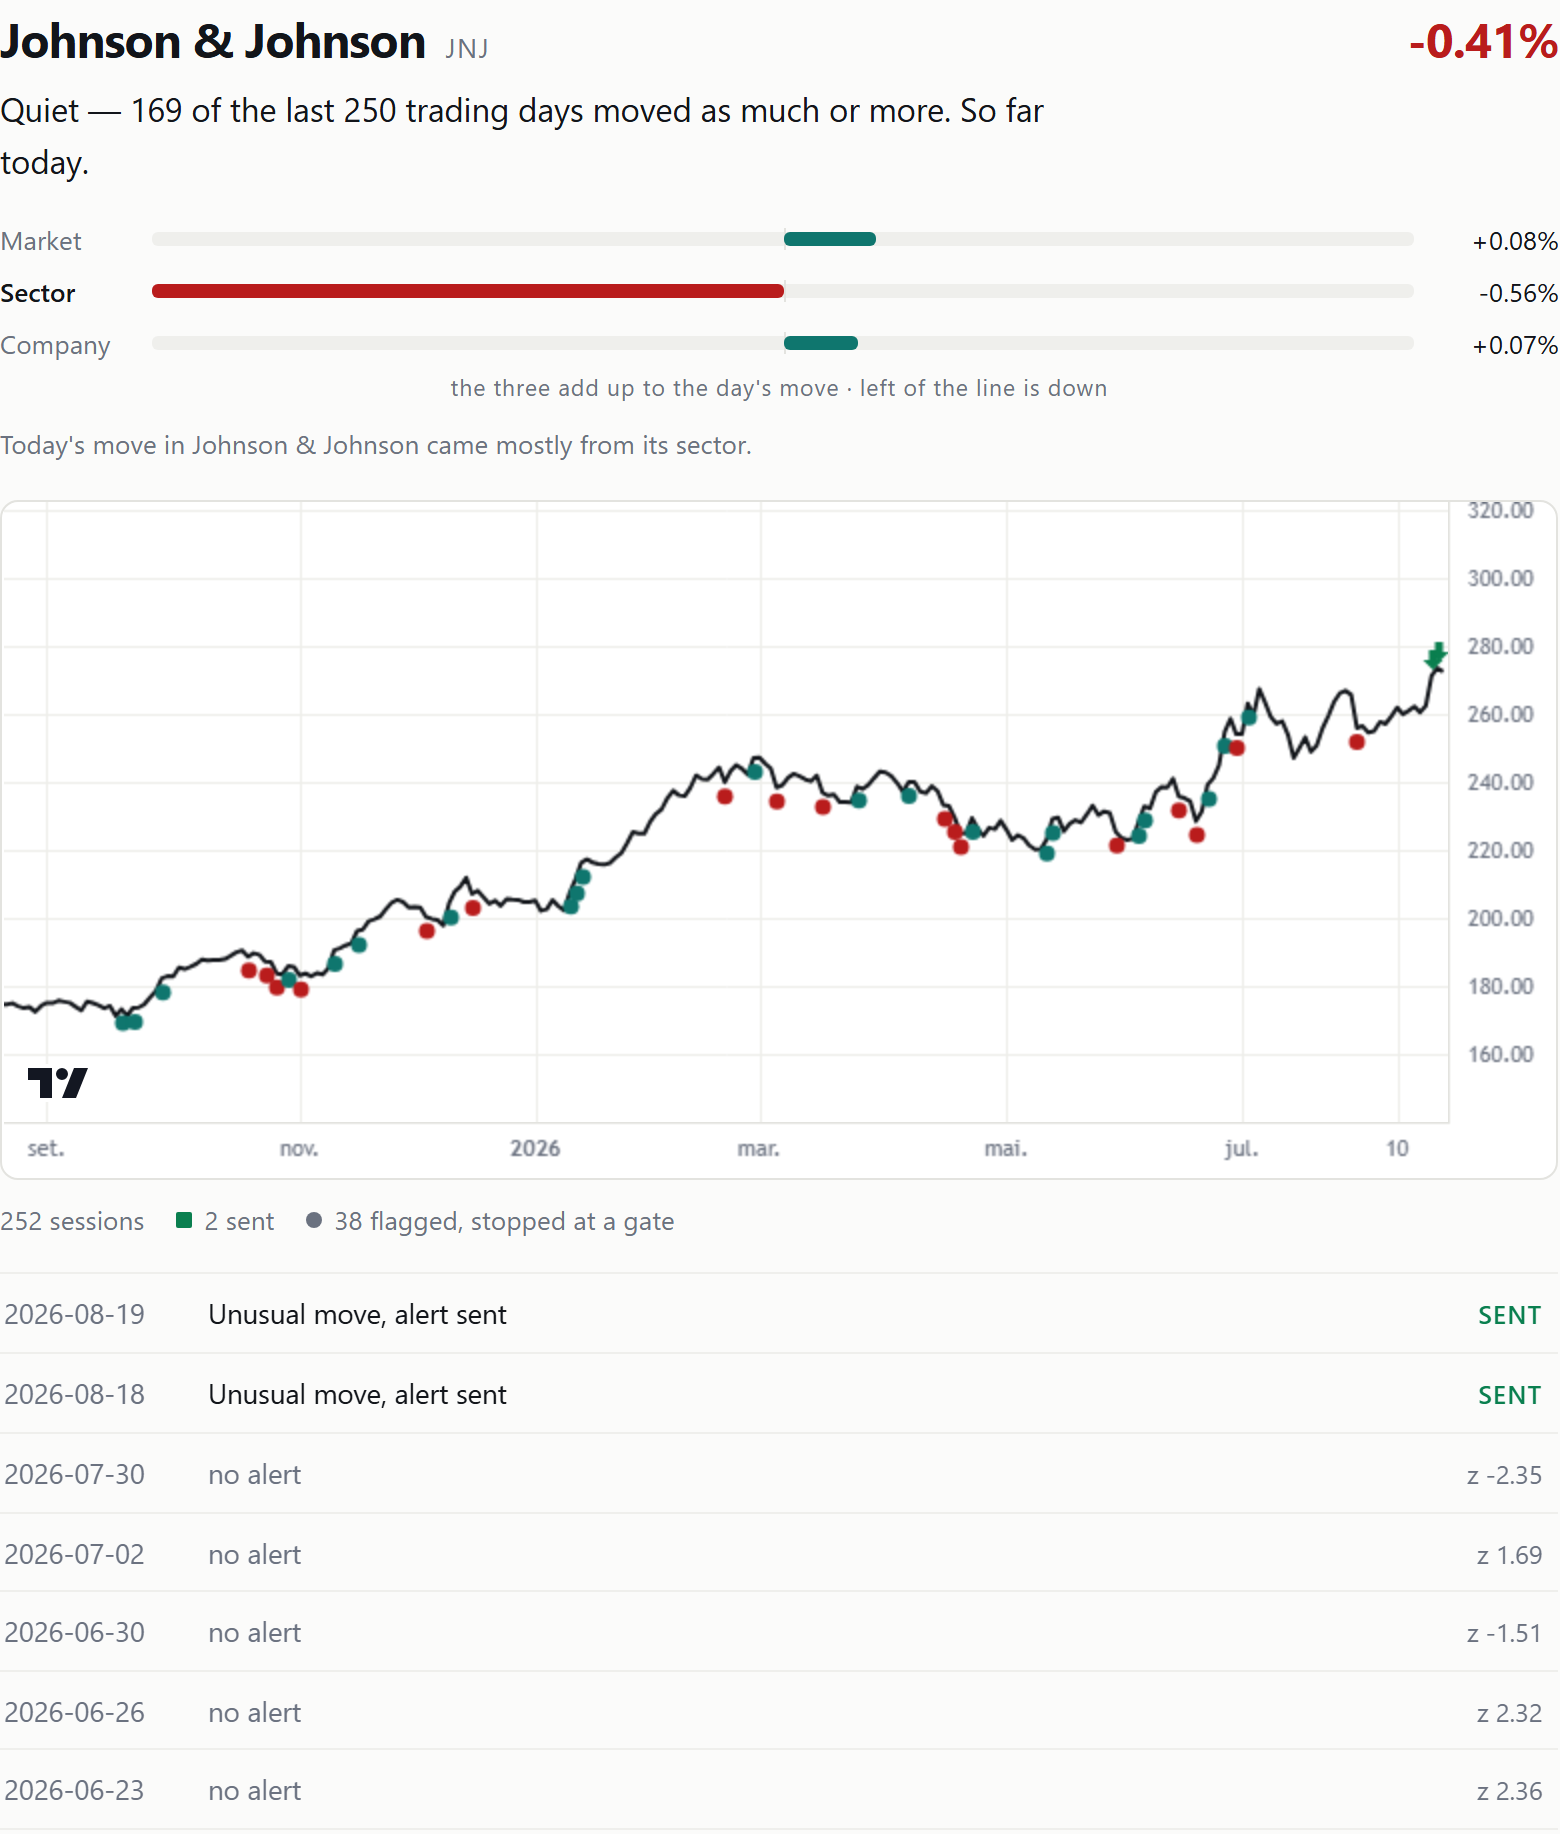
\includegraphics[width=0.70\textwidth]{figures/app_v6_empresa.png}

\vspace{3mm}
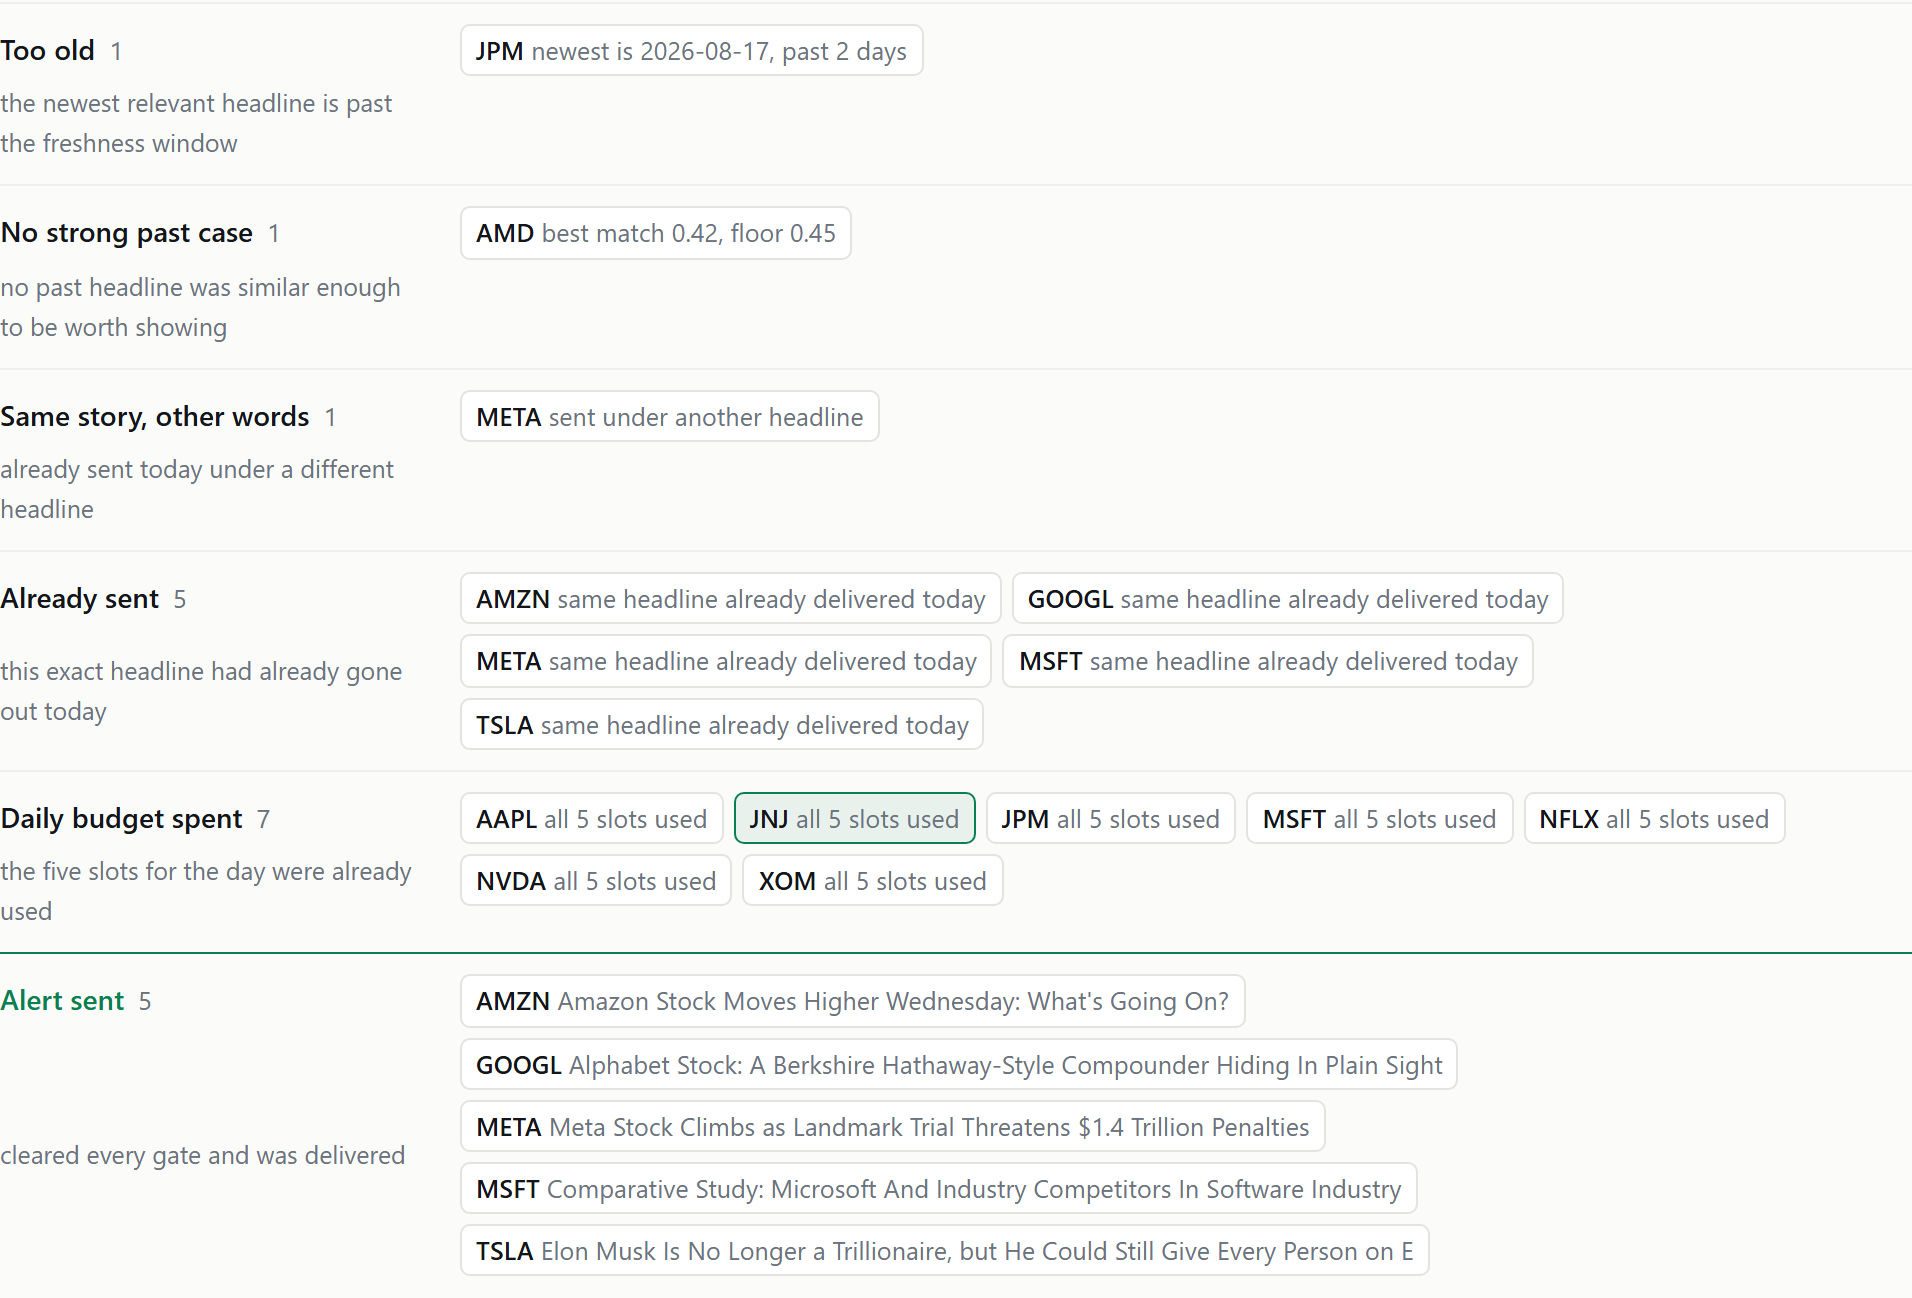
\includegraphics[width=0.86\textwidth]{figures/app_v6_silencio.png}
\caption[A página, capturada em funcionamento]{A página, capturada da aplicação em
funcionamento a 20 de agosto de 2026, com a sessão americana a decorrer.
\textbf{Em cima}, uma empresa. \textbf{Em baixo}, as
decisões do dia inteiro, pela ordem por que são tomadas, com a margem que faltou quando
existe.}
\label{fig:sis_pagina}
\end{figure}

Uma nota sobre o número que aparece na última linha do alerta. Os $57\%$ não são a pontuação em bruto
do modelo: são o resultado de a converter numa \emph{probabilidade}, ajustando uma sigmoide sobre um
bloco de validação reservado \autocite{niculescu2005calibration}. A distinção não é decorativa neste
contexto. Uma pontuação em bruto ordena bem e não significa nada por si, ao passo que uma
probabilidade calibrada pretende que, entre os títulos a que o sistema atribui $57\%$,
aproximadamente essa fração tenha mesmo um movimento invulgar. É a diferença entre um número que se
pode mostrar a alguém e um número que só serve por dentro.

Convém, porém, não prometer mais do que se cumpre. A Secção~\ref{sec:av_qi3} reporta o erro médio
desta probabilidade, mas a Secção~\ref{sec:met_conta} regista uma limitação que esse erro médio não
revela: a calibração é ajustada num bloco com mais casos importantes do que aquele a que é aplicada,
e por isso o valor anunciado é cerca de cinco pontos percentuais otimista. A ordenação entre notícias
não é afetada, porque a transformação preserva a ordem; o número absoluto é.

\paragraph{O que o alerta afirma, e o que a medição sustenta.}
Os três precedentes têm o \emph{mesmo} impacto, $-2.73\%$, e a mesma data. Não é coincidência: o
impacto é medido por \textbf{(empresa, dia)}, logo três títulos da mesma empresa no mesmo dia
partilham o mesmo valor por construção. A frase ``\emph{3 of 3 shown cases moved down}'' apresenta
como concordância entre três casos aquilo que é \textbf{um dia observado três vezes}.

Medido sobre os $247$ alertas de notícia com precedentes já entregues: em $36.8\%$ deles os casos
mostrados assentam em menos dias distintos do que casos exibidos, e em $11.3\%$ os três são o
mesmo dia. Dos $120$ alertas que afirmam unanimidade, $23.3\%$ apoiam-se num único dia.

Isto \textbf{não afeta} nenhum número reportado no Capítulo~\ref{cap:avaliacao}: a precisão@5 conta
títulos e a concordância de direção é medida par a par sobre o corpus histórico. Afeta a força que
o \emph{alerta} reivindica quando fala ao utilizador, e fica registado como limitação por isso.

E a garantia que sustenta tudo isto é de construção, não de boa vontade: \textbf{cada número do
texto vem do objeto que o calculou}. O texto é montado a partir dessas peças. Não é possível o alerta
dizer $+4.47\%$ e o sistema ter calculado outro valor, porque só existe um sítio onde esse valor
existe.

\section{Onde o sistema corre, e com que latência}
\label{sec:sis_implantacao}

O sistema corre como processo permanente, com um ciclo de varredura de sessenta segundos, sobre
créditos de alojamento incluídos no plano académico. A primeira versão usava um agendador gratuito
de melhor esforço, que na prática corria de hora e meia em hora e meia; a mudança para um processo
permanente foi feita para reduzir o atraso dos alertas, e a Tabela~\ref{tab:sis_latencia} mede o
que ela comprou.

\begin{table}[!htbp]
\caption[O que o ciclo de 60 segundos comprou]{Latência medida sobre os alertas entregues. As duas
primeiras linhas separam as duas eras; as duas últimas repartem o percurso e são medidas sobre o
conjunto \emph{inteiro}, as duas eras juntas, e por isso não se subtraem às de cima. O tempo está
quase todo na \emph{descoberta}, não na entrega.}
\label{tab:sis_latencia}
\centering
\begin{tabular}{p{0.46\textwidth} r r}
\toprule
\tabhead{Medição} & \tabhead{Valor} & \tabhead{Casos} \\
\midrule
\multicolumn{3}{l}{\emph{Por era, sobre o percurso completo}} \\
Mediana, com o agendador gratuito & $196$ min & $28$ \\
Mediana, com o ciclo de 60 segundos & $143$ min & $73$ \\
\midrule
\multicolumn{3}{l}{\emph{As duas eras juntas, repartindo o percurso}} \\
Da publicação até o sistema detetar & $\approx 158$ min & $101$ \\
Da deteção até a mensagem chegar & $\approx 1$ s & $101$ \\
\bottomrule
\end{tabular}
\end{table}

As duas eras diferem em $53$ minutos de mediana. Essa diferença não isola o efeito do ciclo: as
duas eras não correram em paralelo, entre elas mudaram as fontes de notícias e o período de
calendário, e as amostras são de $28$ e $73$ casos sem intervalo de confiança. O que a medição
mostra com segurança é a repartição do percurso, e essa não depende da comparação entre eras:
\textbf{quase todo o tempo decorre até a notícia aparecer na fonte gratuita}, e a entrega demora
cerca de um segundo depois de o sistema a ver.

A latência é, portanto, uma limitação das fontes e não da infraestrutura. Um serviço pago de
notícias em tempo real resolveria-a, e violaria a restrição de custo nulo que define o âmbito
deste trabalho.

\subsection{A base de casos cresce com o que o sistema observa}
\label{sec:sis_ciclo}

Todo o título relevante que a varredura vê é guardado como candidato a precedente. Oito dias
depois, quando o impacto no preço já é observável, esse candidato é medido com a mesma regra de
alinhamento da Secção~\ref{sec:met_recuperacao} e entra na base de casos. A espera não é uma
ineficiência: é o que impede um caso de conhecer o seu próprio desfecho. A Figura~\ref{fig:sis_ciclo_kb}
mostra o ciclo.

\begin{figure}[ht]
\centering
\begin{tikzpicture}[font=\footnotesize, >={Stealth[length=2.2mm]},
  et/.style={draw, rounded corners=3pt, align=center, inner sep=4pt, text width=2.65cm,
             minimum height=1.25cm, fill=black!5},
  esp/.style={draw, dashed, rounded corners=3pt, align=center, inner sep=4pt, text width=2.4cm,
              minimum height=1.25cm, fill=white},
]
  \node[et]  (a) at (0,0)     {\textbf{hoje}\\ a varredura vê um título relevante};
  \node[esp] (b) at (3.55,0)  {guardado como \emph{candidato}, com o seu vetor};
  \node[et]  (c) at (7.0,0)   {\textbf{oito dias depois}\\ o preço já disse o que fez};
  \node[et]  (d) at (10.5,0)  {entra na \textbf{base de casos} como precedente};

  \draw[->, thick, black!55] (a) -- (b);
  \draw[->, thick, black!55] (b) -- (c);
  \draw[->, thick, black!55] (c) -- (d);

  % o regresso: a base alimenta a varredura seguinte
  \draw[->, thick, black!55] (d.south) -- ++(0,-0.85) -| (a.south)
    node[pos=0.25, below, font=\scriptsize, black!65]
    {os alertas de amanhã comparam-se com o que o sistema viu ontem};

  \node[align=left, font=\scriptsize, text=black!60, text width=3.2cm] at (5.3,1.55)
    {a espera não é uma ineficiência: é o que impede o caso de conhecer o seu próprio futuro};
\end{tikzpicture}
\caption[O ciclo que faz a base de casos crescer]{O que acontece a um título entre ser visto e
poder servir de precedente. A espera de oito dias existe porque o impacto de um caso só é
observável depois de o preço se mover, e medi-lo antes seria deixar o caso conhecer o seu próprio
desfecho. Este ciclo mantém atualizada a \textbf{evidência} que o sistema mostra, e não os pesos do
modelo: nada aqui re-treina nada.}
\label{fig:sis_ciclo_kb}
\end{figure}

Este mecanismo mantém atualizada a \emph{evidência} que o sistema mostra, e não os pesos do
modelo: nada aqui re-treina nada. Da taxonomia de deriva de conceito \autocite{gama2014survey},
o sistema tem a deteção da mudança e não tem a adaptação a ela.

Verificou-se, já com o sistema em funcionamento, que este ciclo tinha estado parado dezanove dias
sem que nenhum erro fosse registado: os dois processos correm em máquinas separadas cujo disco é
apagado a cada reinício, e os ficheiros de maturação não estavam a ser publicados no repositório de
dados. É a classe de custo que \textcite{sculley2015debt} descrevem como dependência de dados não
declarada, cada peça cumpre o seu contrato e a suposição que as liga não está escrita em lado
nenhum. O Capítulo~\ref{cap:conclusoes} retoma-a como limitação.

A base implantada tem $38\,214$ casos com impacto medido, guardados como matriz de precisão
simples mapeada do disco. O formato importa: os mesmos vetores em estruturas nativas de Python
excediam a memória do contentor, e a mudança de formato foi o que permitiu usá-los. O efeito no
produto é o que se esperaria de multiplicar a base por vinte, com os precedentes exibidos a passarem
a ser da própria empresa e sobre o mesmo assunto.

\section{O ciclo de vida do modelo, e o que nele é meu}
\label{sec:sis_ciclo_vida}

É uma pergunta justa, e merece uma resposta reunida num sítio só, porque as peças estão espalhadas
por três capítulos e obrigar quem lê a juntá-las é uma forma de não responder.

Começo pela parte incómoda. Este sistema treina \textbf{um} modelo, e esse modelo é uma regressão
logística com nove entradas que, medida contra uma linha de base de uma só variável,
\textbf{perdeu}. Se a pergunta for \emph{quantos modelos treinou?}, a resposta é um, e é pequeno.

A engenharia não está no tamanho do modelo. Está no que foi preciso construir para que aquele
número, e a conclusão negativa que ele sustenta, sejam de confiança. Essa construção tem sete peças,
e cada uma existe porque a sua ausência produziria um resultado bonito e falso.
A Figura~\ref{fig:sis_lifecycle} mostra as duas metades do ciclo.

\begin{figure}[ht]
\centering
\begin{tikzpicture}[font=\scriptsize, >={Stealth[length=2mm]},
  cx/.style={draw, rounded corners=2pt, align=center, inner sep=3pt, text width=2.15cm,
             minimum height=1.0cm, fill=black!5},
  art/.style={cx, fill=black!14, draw=black!55, thick},
  obs/.style={cx, fill=white, draw=black!45},
  fase/.style={font=\scriptsize\bfseries, text=black!60},
]
  \node[fase] at (-1.55,0.95) {construir};
  \node[cx]  (d) at (0,0)    {conjunto de dados\\ rotulado};
  \node[cx]  (t) at (2.5,0)  {treino};
  \node[cx]  (v) at (5.0,0)  {validação\\ \emph{calibração}};
  \node[cx]  (s) at (7.5,0)  {teste\\ \emph{uma só vez}};
  \node[art] (m) at (10.0,0) {artefacto\\ versionado};

  \foreach \xa/\xb in {d/t, t/v, v/s, s/m} \draw[->, thick, black!55] (\xa) -- (\xb);

  \node[fase] at (-1.55,-1.75) {observar};
  \node[art] (p) at (0,-1.9)   {o \textbf{mesmo} modelo, em produção};
  \node[obs] (g) at (2.5,-1.9) {registo de cada decisão};
  \node[obs] (w) at (5.0,-1.9) {esperar que o preço responda};
  \node[obs] (r) at (7.5,-1.9) {pós-validação\\ e deriva};

  \draw[->, thick, black!55] (m.south) -- ++(0,-0.5) -| (p.north);
  \foreach \xa/\xb in {p/g, g/w, w/r} \draw[->, thick, black!55] (\xa) -- (\xb);

  % o elo que NAO existe
  \draw[->, dashed, black!40] (r.east) -- ++(0.9,0) |- (10.0,-1.05)
    node[pos=0.72, right, align=left, text width=2.2cm, black!55]
    {re-treino:\\ \textbf{não existe}};
\end{tikzpicture}
\caption[O ciclo de vida do modelo]{As duas metades do ciclo. Em cima, construir: os dados são
rotulados, a divisão é cronológica, a calibração é ajustada na validação, e o bloco de teste é
usado no fim. Em baixo, observar: o modelo que corre é o mesmo que foi avaliado, cada decisão fica
registada, e dias depois é confrontada com o que o preço realmente fez. O elo a tracejado é o que
fecharia o ciclo e \textbf{não existe}: a deriva é medida e não corrigida, e a
Secção~\ref{sec:con_futuro} diz o que faria falta para a corrigir.}
\label{fig:sis_lifecycle}
\end{figure}

\begin{description}
  \item[1. O conjunto de dados é construído, não encontrado.] O \gls{FNSPID} dá títulos com data;
        os preços vêm de outro lado. Alinhar as duas coisas, decidir a que dia de negociação
        pertence uma notícia de sábado, e derivar o rótulo a partir do movimento futuro, é o
        trabalho que produz as $79\,753$ linhas da Secção~\ref{sec:met_dados}. Nenhuma delas existia
        antes.

  \item[2. O rótulo é uma decisão, e é declarado como tal.] ``Houve movimento anormal nos três dias
        seguintes'' não é um facto que estivesse nos dados: é uma definição, com um limiar e um
        horizonte escolhidos por quem constrói. Por isso a Secção~\ref{sec:av_qi3} não se fica
        por essa escolha e mede \textbf{nove} definições alternativas.

  \item[3. A separação temporal é imposta por um teste, não prometida.] A divisão é cronológica com
        embargo, e existe um teste automático que altera o futuro de um exemplo e exige que as
        entradas fiquem iguais e o rótulo mude. É a diferença entre afirmar que não há fuga e ter
        onde a ir buscar se houver.

  \item[4. As probabilidades são calibradas, e o seu enviesamento está medido.] O modelo devolve um
        número entre zero e um, e esse número é usado para ordenar e para cortar. A calibração de
        Platt é ajustada num bloco reservado, e o Capítulo~\ref{cap:avaliacao} declara que a
        prevalência da validação não é a do teste, o que desloca a escala.

  \item[5. Os artefactos existem e estão versionados.] O modelo treinado, o calibrador e um ficheiro
        que descreve a corrida (dimensão de cada bloco, prevalência, semente, métricas) vivem
        no repositório. Uma métrica sem o artefacto que a produziu não é reproduzível; é uma
        afirmação.

  \item[6. O modelo implantado é o modelo avaliado.] Isto parece trivial e não é. O codificador de
        frases usado na avaliação corre sobre uma biblioteca pesada que não cabe no contentor de
        produção. Em vez de trocar por outro modelo, o que faria a dissertação descrever um
        sistema que ninguém usa, exportou-se o \emph{mesmo} modelo para um formato leve, e mediu-se
        a fidelidade da conversão. A alternativa fácil era mais rápida e teria invalidado o
        Capítulo~\ref{cap:avaliacao}.

  \item[7. O que corre é observado.] Cada decisão de triagem é registada. Dias depois, quando o
        preço já disse o que fez, um segundo procedimento rotula essas decisões com a mesma regra do
        treino e mede se o modelo está a ajudar. Foi assim que se soube que \emph{não} está, e é a
        Secção~\ref{sec:av_qi3} que o reporta. A deriva das entradas é medida pelo mesmo espírito.
\end{description}

\subsection{O que é meu, e o que é consumido}

A distinção interessa, e escondê-la seria fácil.

\textbf{Consumido de fora:} um codificador de frases pré-treinado, e mais nada em matéria de
modelos. Não foi ajustado, não foi treinado, e o trabalho não reivindica nada sobre ele além de o
ter escolhido \emph{por medição}, contra quatro alternativas: um modelo maior, dois codificadores
mais recentes, e um modelo específico de finanças, que foi o pior de todos. É uma dependência \textbf{essencial}: sem representação de frases não há
recuperação semântica. É também \textbf{substituível}: a interface que o isola tem uma
implementação de reserva que degrada para sobreposição de palavras quando o modelo não está
disponível.

\textbf{Construído aqui:} o conjunto de dados rotulado, o alinhamento anti-fuga, o detetor e a sua
janela protegida, a decomposição com encolhimento, a base de casos com impacto medido, o modelo de
triagem e a sua calibração, as portas de decisão com as constantes derivadas, a camada de explicação
amarrada aos objetos calculados, e o ciclo de observação que mede o sistema depois de implantado.

\textbf{Deliberadamente ausente:} não há aqui um modelo de linguagem a escrever texto para o
utilizador, pela razão que a Secção~\ref{sec:ctx_llm} desenvolve e que atravessa o trabalho: uma
frase gerada é uma afirmação, e este sistema entrega afirmações com a evidência ao lado.

\subsection{O que este ciclo não tem}

Duas coisas, e as causas são diferentes.

\textbf{Não há re-treino.} Os pesos são de 2018--2023 e não voltaram a ser ajustados, apesar de a
deriva estar medida. Seria possível, porque os rótulos novos vêm dos preços: o que impede não é a
técnica, é que re-treinar com o registo de produção mudaria os números que este documento reporta,
e isso precisa de tempo para ser avaliado. Fica como trabalho declarado.

% \looseness=-1 pede ao TeX que componha o paragrafo uma linha mais curto. Esta aqui por
% composicao e nao por estilo: sem ele o capitulo transbordava duas linhas para uma pagina
% so delas, que se le como um erro de composicao. So se ve a renderizar.
\looseness=-1
\textbf{Não há verdade humana.} Os três rótulos deste trabalho, ou seja movimento anormal, mesmo
setor e percentil de movimento, são aproximações verificáveis que nunca foram confrontadas com o
julgamento de uma pessoa. É a limitação de que mais dependem as outras, e o
Capítulo~\ref{cap:conclusoes} volta a ela.
